\documentclass[man]{apa7}
\usepackage[american]{babel}
\setcounter{tocdepth}{4}
\setcounter{secnumdepth}{4}
\usepackage{csquotes}
\usepackage{titlepic}
\usepackage{graphicx}
\usepackage{adjustbox}
\usepackage{pdfpages}
\usepackage{hyperref}
\hypersetup{
    colorlinks=true,
    linkcolor = blue,      
    urlcolor=blue
    }
\usepackage{amsfonts}
\usepackage[style=apa,backend=biber]{biblatex}
\usepackage{lipsum}
\DeclareLanguageMapping{american}{american-apa}
\addbibresource{mybibfile.bib}
\usepackage{fancyhdr}
\pagestyle{fancy}
\fancyhf{}
\lhead{\textit{Word Embeddings and Language Trees}}
\rhead{\thepage}


\begin{document}
\begin{titlepage}
\centering
{\large \textbf{ Istanbul Technical University - Science and Letters Faculty}}\\
{\large \textbf{Mathematics Engineering Program}}\\[4\baselineskip]

\includegraphics[scale = 1.5]{itülogo.png}\\[6\baselineskip]
{\LARGE \textbf{Word Embeddings and Language Trees}}\\[2\baselineskip]

{\Large Student Name: Arif Çakır}\\
{\large Student Number: 090190355}\\
{\large Course: MAT4091E}\\
{\large Advisor: Prof. Dr. Atabey Kaygun}\\
{\large Submission Date: June 11, 2023}\\
\end{titlepage}
\tableofcontents
\pagebreak

\section{Introduction}
Language is a fundamental aspect of human communication and one of the most common ways to pass on information and culture throughout history. Due to their nature of encapsulating information, different languages are studied by linguists throughout the years. Thanks to this scientific foundation, machine learning, and computer science are also advanced upon this topic. Natural Language Processing (NLP) is the subfield of machine learning that studies the processing of human language by computers. One of the most popular NLP techniques in recent years is Word Embedding, which represents words as vectors in semantic space that allows applying mathematical operations on them to analyse. Word Embedding can be used on various subjects such as text classification, translation, and sentiment analysis with promising results. It is aimed in this paper to study several Word Embedding techniques and their applications. The aim is to create a model by applying various Word Embedding models and with the help of this model, describing the relationships and similarities of languages.

The rest of the paper is organised as follows: In Section 2, word embedding techniques are discussed. The word embedding techniques that analysed on the paper are Term Frequency (TF), Inverse Document Frequency (IDF), Skip-Gram, Continuous Bag of Words (CBOW), Global Vectors of Word Representation (GloVe), and Bidirectional Encoder Representations from Transformers (BERT). Section 2 is followed by Section 3 which discusses the Word2Vec method. After that, Section 4 introduces the dataset The Divine Comedy by Dante Alighieri. Also in Section 4, Skip-Gram and CBOW models are applied to the dataset. This application aims to create a dendrogram of cosine similarity of languages, which clusters languages based on their similarities. This is followed by Section 5, which discusses the output of Section 4. Finally, the paper is concluded in Section 6.

\section{Word Embedding Techniques}
Word Embedding is one of the most popular natural language processing techniques due to its vector representation of the words. As Agarwal stated, capturing the semantic meaning of the words in a vector of text is the ambition of the word embedding techniques (Agarwal, 2022). With respect to that, some of the most popular word embedding techniques will be studied in this section. Those techniques are TF, which counts the rarity of words; IDF, which counts the rarity of words; Skip-Gram method, which is used by Word2Vec; Continuous Bag of Words method, also used by Word2Vec;  GloVe, which captures co-occurrence of words; and BERT, a family of masked-language models introduced by Google.

\subsection{Term Frequency - Inverse Document Frequency}
Term Frequency (TF) is a word embedding technique which counts the occurrence of the words in a document. TF can be shown as

\begin{equation}
TF(i) =   \frac{\log(Frequency(i,j))}{\log(TotalNumber(j))}.
\end{equation}

where $Frequency(i,j)$ is the frequency of a word that occurred in a j word document and $TotalNumber(j)$ is the total number of the words in the document.

On the other hand, Inverse Document Frequency (IDF) is practically the opposite of the TF method. In this method, the algorithm relies on the information gained from the words which are rarely used. IDF can be written as

\begin{equation}
IDF (i) = \log (\frac{TotalNumber(j)}{Frequency(j,i)}).
\end{equation}

where $Frequency(i,j)$ is the frequency of a word that occurred in a j word document and $TotalNumber(j)$ is the total number of the words in the document.

TF-IDF mainly shows the degree of relevancy of word i in document j, while the main disadvantage of TF-IDF is it does not grasp the contextual relationship between the words. As Kınık and Güran stated, TF-IDF does not capture semantic relationships between words and accepts them as independent values (Kınık and Güran, 2021). Due to TF-IDF's lack of capturing the semantic relationship of the words, TF-IDF is mainly used to detect stop words.

\subsection{Skip-Gram Algorithm}
The Skip-Gram model is used by word embedding tasks of the Word2Vec model, which will be discussed in the following chapters. Dive Into Deep Learning (n.d) states that a word can be used for generating its surrounding words in the Skip-Gram model. For example, if the sentence "the man loves his son" is taken and "loves" is chosen as the center word, then the Skip-Gram model considers the conditional probability for generating the words. This architecture can be seen in \textbf{Figure 1}. Due to this approach, each word has a two-dimensional vector representation in the Skip-Gram model. 

\begin{center}

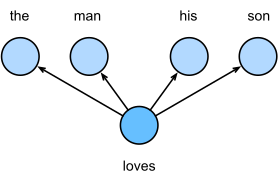
\includegraphics[scale=1]{skip-gram.png}

\textbf{Figure 1:} Skip-Gram model architecture, from Dive Into Deep Learning\\[2\baselineskip]

\end{center}

Dive Into Deep Learning continues that, for any word with index $\mathit{i}$ in the directory, $\mathbf{v_\mathit{i}} \in \mathbb{R}^d$ and $\mathbf{u_\mathit{i}} \in \mathbb{R}^d$ are its two vector representations, where $\mathbf{v_\mathit{i}}$ is when the word is used as the "center word" and $\mathbf{u_\mathit{i}}$ is when the word is used as the "context word". If $\mathit{w_o}$ is any context word and $\mathit{w_c}$ is given center word, then conditional probability of generating $\mathit{w_o}$ can be modelled as

\begin{equation}
P(w_o | w_c) = \frac{exp(\mathbf{u_\mathit{o}}^\top \mathbf{v_\mathit{c}})}{\sum_{i \in \mathcal{V}} exp(\mathbf{u_\mathit{i}}^\top \mathbf{v_\mathit{c}})}.
\end{equation}

where $ \mathcal{V}$ is the vocabulary index set. If a text sequence of length $T$ is given and word at time step $t$ is denoted as $\mathit{w}^t$, then the likelihood function of the Skip-Gram model for context widow size $m$ is as follows:

\begin{equation}
\prod_{t=1}^T \prod_{-m \le j \le m , j \neq 0} P(w^{t+j} | w^t).
\end{equation}

The Skip-Gram model parameters are the center word and context word vector for each word in the corpus. In order to train the Skip-Gram model, the given loss function must be minimized:

$$ -\sum_{t=1}^T \sum_{-m \le j \le m, j \neq 0} logP(w^{(t+j)} | w^{(t)}).$$

Moreover, while using (stochastic) gradient descent to minimize the loss function, gradients of log conditional probability must be obtained. For center word $w_c$ and context word $w_o$, log conditional probability is

\begin{equation}
logP(w_o|w_c) = \mathbf{u}_o^\top \mathbf{v}_c - log(\sum_{i \in \mathcal{V}} exp(\mathbf{u}_i^\top \mathbf{v}_c)).
\end{equation}

And the gradient of center word $\mathbf{v}_c$ can be obtained as

\begin{equation}
\frac{\partial P(w_o | w_c)}{\partial \mathbf{v}_c} = \mathbf{u}_o - \sum_{j \in \mathcal{V}} P(w_o|w_c)\mathbf{u}_j.
\end{equation}

After this calculation, center word vector $\mathbf{v}_i$ and context word vector $\mathbf{u}_i$ are obtained for index $i$ in the dictionary.

\subsection{Continuous Bag of Words}
The other method for word embedding in Word2Vec is the Continuous Bag of Words (CBOW) method. The main difference between Skip-Gram and CBOW is instead of generating surrounding words with respect to the center word, CBOW generates the center word with the help of surrounding words. If the same example "the man loves his son" is taken for the CBOW model, instead of generating surrounding words based on the center word "loves", the model generates the center word "loves" from its surroundings. This architecture can be seen in \textbf{Figure 2}.
\\[2\baselineskip]

\begin{center}
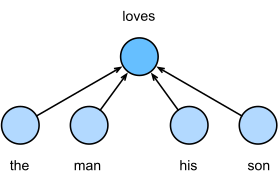
\includegraphics[scale=1]{cbow.png}

\textbf{Figure 2:} CBOW model architecture, from Dive Into Deep Learning\\[2\baselineskip]

\end{center}

According to Dive Into Deep Learning (n.d.), in order to calculate conditional probability, context word vectors are averaged because there are multiple words. For any word with index $i$ in the dictionary, $\mathbf{v_\mathit{i}} \in \mathbb{R}^d$ is the context word while $\mathbf{u_\mathit{i}} \in \mathbb{R}^d$  is the center word. It can be seen that meanings are switched compared to the Skip-Gram model. While $w_o,...,w_{o_{2m}}$ the conditional probability of generating center word $w_c$ can be modelled as following:

\begin{equation}
P(w_c|w_o,...,w_{o_{2m}}) = \frac{exp(\frac{1}{2m}u_c^\top(\mathbf{v}_{o_1}+...+\mathbf{v}_{o_{2m}}))}{\sum_{i \in \mathcal{V}} exp(\frac{1}{2m}u_c^\top(\mathbf{v}_{o_1}+...+\mathbf{v}_{o_{2m}}))}.
\end{equation}

For simplicity, $\mathcal{W}_o = \{ w_o,...,w_{o_{2m}}\}$ and $\bar{\mathbf{v}}_o = (\mathbf{v}_{o_1}+...+\mathbf{v}_{o_{2m}})/(2m)$. The equation given above is simplified as follows:

\begin{equation}
P(w_c | \mathcal{W}_o) = \frac{exp(u_c^\top \bar{\mathbf{v}}_o)}{\sum_{i \in \mathcal{V}} exp(u_i^\top \bar{\mathbf{v}}_o)}.
\end{equation}

Furthermore, Dive Into Deep Learning continues as if the length of a text sequence is $\mathit{T}$ and the word at time $t$ is $w^{(t)}$, then for context window of size $m$ the likelihood function of CBOW model is

\begin{equation}
\prod_{t=1}^T P(w^{(t)}| w^{(t-m)},..., w^{(t-1)},w^{(t+1)},...,w^{(t+m)}).
\end{equation}

Due to CBOW and skip-gram models being similar, training them is also almost the same. According to Dive Into Deep Learning, to train the CBOW model, the maximum likelihood estimation of the CBOW model is equal to the minimization of the following loss function

\begin{equation}
- \sum_{t=1}^T logP(w^{(t)} | w^{t-m)} ,..., w^{(t-1)} ,w^{(t+1)}, ...,w^{(t+m)}).
\end{equation}

where

\begin{equation}
logP(w_c | \mathcal{W}_o) = \mathbf{u}_c^\top \bar{\mathbf{v}}_o - log(\sum_{i \in \mathcal{V}} exp(\mathbf{u}_i^\top \bar{\mathbf{v}}_o)).
\end{equation}

Through differentiation, the following gradient can be obtained

\begin{equation}
\frac{\partial log P(w_c| \mathcal{W}_o )}{\partial \mathbf{v}_{o_i}} = \frac{1}{2m}(\mathbf{u}_c - \sum_{j \in \mathcal{V}} P(w_j| \mathcal{W}_o \mathbf{u}_j)).
\end{equation}

Which is gradient with respect to any context word vector $\mathbf{v}_{o_i}$. 

\subsection{Global Vectors for Word Representation}
Global Vectors for Word Representation (GloVe) is an unsupervised learning algorithm. Unlike Word2Vec, GloVe captures global contextual information of words by calculating a global word-word co-occurrence matrix. For example, in a large corpus, the word "liquid" is more likely to co-occur with "water" than "ice", but the word "solid" is more likely to co-occur with "ice" than "steam". According to Agarwal, only the local context of words is captured by Word2Vec (Agarwal, 2022). On the other hand, the entire corpus is considered by GloVe, and a large matrix that can capture the co-occurrence of words within the corpus is created.
\\[2\baselineskip]

\begin{center}
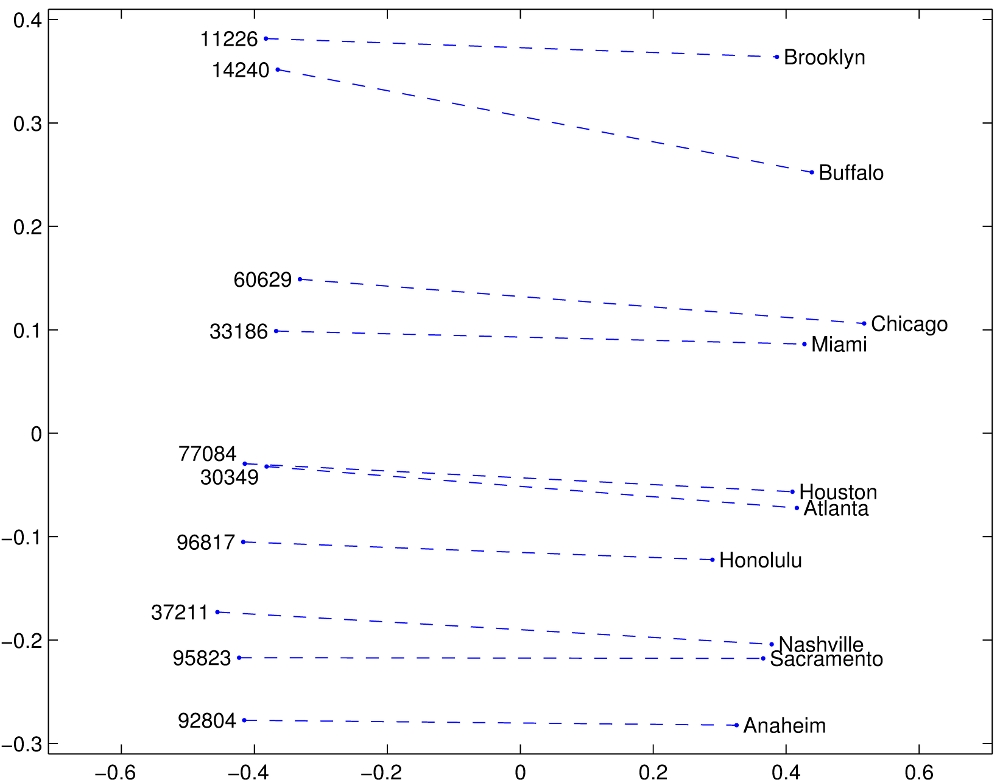
\includegraphics[scale=3]{city_zip.jpg}

\textbf{Figure 3:} GloVe vectors capturing the relation between city and zip code, from Stanford University\\[2\baselineskip]

\end{center}

Agarwal continues by GloVe has the combination of the advantages of two-word vector learning methods: matrix factorization like latent semantic analysis (LSA) and local context window method (like Skip-Gram or CBOW). LSA is the technique that analyses the relationship between a set of documents and the terms they contain by using singular value decomposition. 

Furthermore, the GloVe method's computational time is reduced by a rather simpler least square error function. As it is stated in Dive Into Deep Learning, Glove makes three changes to the Skip-Gram model square loss (n.d.). where vectors $\mathbf{v_\mathit{i}} \in \mathbb{R}^d$ and $\mathbf{u_\mathit{i}} \in \mathbb{R}^d$ keep same representations as the Skip-Gram model, those their changes are as following:

1. Using variables $p'_{ij} = x_{ij}$ and $q'_{ij} = exp(\mathbf{u}_j^\top \mathbf{v}_i)$ that are not probabilistic distributions. After taking their logarithms, the squared loss term becomes $(log(p'_{ij})-log(q'_{ij}))^2 = (\mathbf{u}_j^\top \mathbf{v}_i - log (x_{ij}))^2$.

2. For each word $w_i$, adding two scalar model parameters: the center word bias $b_i$ and context word bias $c_i$.

3. Replacing the weight of each loss term $h(x_{ij}$ where $h(x)$ is increasing in the interval of $[0,1]$.
 
Therefore, the loss function of GloVe is:
\begin{equation}
\sum_{i \in \mathcal{V}} \sum_{j \in \mathcal{V}} h(x_{ij})(u_j^\top \mathbf{v}_i + b_i +c_j -log(x_{ij}))^2
\end{equation}


Where suggested choice for $h(x)$ is if $x < c$ , then $h(x) = (x/c)^\alpha$, else $h(x) = 1$. 

Finally, when compared to Word2Vec GloVe handles out of vocabulary words better. Due to that, GloVe performs better in word analogy and named entity recognition tasks.

\subsection{Bidirectional Encoder Representations from Transformers}
Bidirectional Encoder Representations from Transformers (BERT) is a family of masked-language models. Before discussing BERT; the terms context-independent, context-sensitive, task-specific, and task-agnostic must be discussed.

A context-independent function $f(x)$ only takes token $x$ as its input. Due to the complex semantics and synonyms in natural languages, context-independent representations miss the meaning of the words in some cases. For example, the word "bank" can be used in both the sentence "I sat by the bank and enjoyed the view of the river." and the sentence I went to the bank to deposit some money". A context-independent algorithm might miss the difference between these cases.

On the other hand, the context-sensitive function $f(x,c(x))$ is dependent on both token $x$ and context $c(x)$. According to Dive Into Deep Learning, some of the most popular context-sensitive representations are language-model-augmented sequence tagger (TagLM), Context Vectors (CoVe), and ELMo (Embeddings from Language Models).

When it comes to task-specific and task-agnostic representation, task-specific representation is when a model is optimized for a specific task, while task-agnostic representation is when a model is independent of a task-based architecture. For instance, ELMo is a task-specific solution while it is not necessary to create specific architecture for each NLP task. The Generative Pre-Training  (GPT) model is a context-sensitive, task-agnostic representation. However, according to Dive Into Deep Learning, GPT only looks left to right because of the autoregressive nature of natural languages. For example, the sentences "A crane is flying." and "A crane is crashed." is taken, because of word "crane" is sensitive to the context on its left, and GPT will return the same representation of "crane".

Both ELMo and GPT fail in some cases. According to Dive Into Deep Learning (n.d.), the combination of both representations BERT, encodes context bidirectionally and requires minimal architecture changes for a wide range of natural language processing tasks. Differences between ELMo, GPT, and BERT can be seen in \textbf{Figure 4}.
\\[2\baselineskip]

\begin{center}
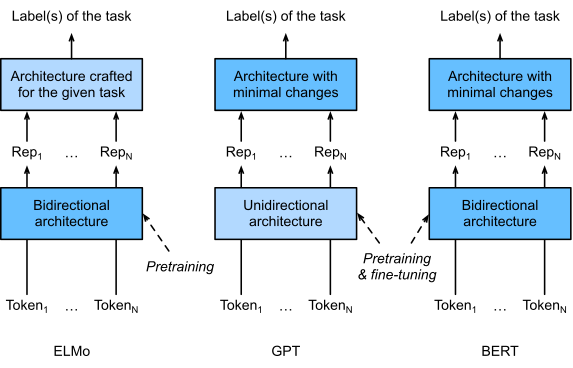
\includegraphics[scale=0.6]{elmo-gpt-bert.png}

\textbf{Figure 4:} Difference between ELMo, GPT, and BERT, from Dive Into Deep Learning\\[2\baselineskip]
\end{center}

Furthermore, Dive Into Deep Learning continues by using a pretrained transformer encoder, any token based on its bidirectional context can be represented by BERT. Furthermore, BERT is similar to GPT in two aspects during supervised learning of downstream tasks.

1. BERT representations will be fed into an added output layer with minimal changes to the model architecture. 

2. while the additional output layer will be trained from scratch, all the parameters of the pre-trained transformer encoder are fine-tuned.

Finally, Agarwal states that there are two variants of BERT: BERT-Base and BERT-Large. While BERT-Base has 110 million parameters, BERT-Large has 340 million parameters.

\section{Word2Vec}
In this section, another natural language processing technique Word2Vec is discussed. As stated in Gensim documentations (n.d.), words are embedded in lower-dimensional vector space by Work2Vec. The method used to compress data into lower dimensions is called autoencoding. After that, in this vector space, vectors which have similarities of context between them are close to each other while words that have different meanings are distant to each other. Word2Vec Model calculates the cosine similarity of those words in order to find relations between them. Due to that, the term autoencoders are discussed and it is followed by a discussion of the Word2Vec model in this section.

\subsection{Autoencoders}

In order to understand the Word2Vec model, the term autoencoders must be discussed. An autoencoder reduces input into lower dimensional data by using neural networks, basically compressing them. After that, this reduced form code can be used in code, which might contain mathematical operations or data analysis. Finally, processed data is decoded by a decoder to get an output that has the same size as the input. Simplilearn states that there are five types of autoencoders (Simplilearn, 2023). Those autoencoders are under complete autoencoders, sparse autoencoders, contractive autoencoders, denoising autoencoders, and variational autoencoders.
Due to being a method for processing non-mathematical data, Autoencoders are mainly used in tasks like anomaly detection, feature detection, facial recognition, and word embedding. The typical structure of an autoencoder can be seen in \textbf{Figure 5}.\\

\begin{center}

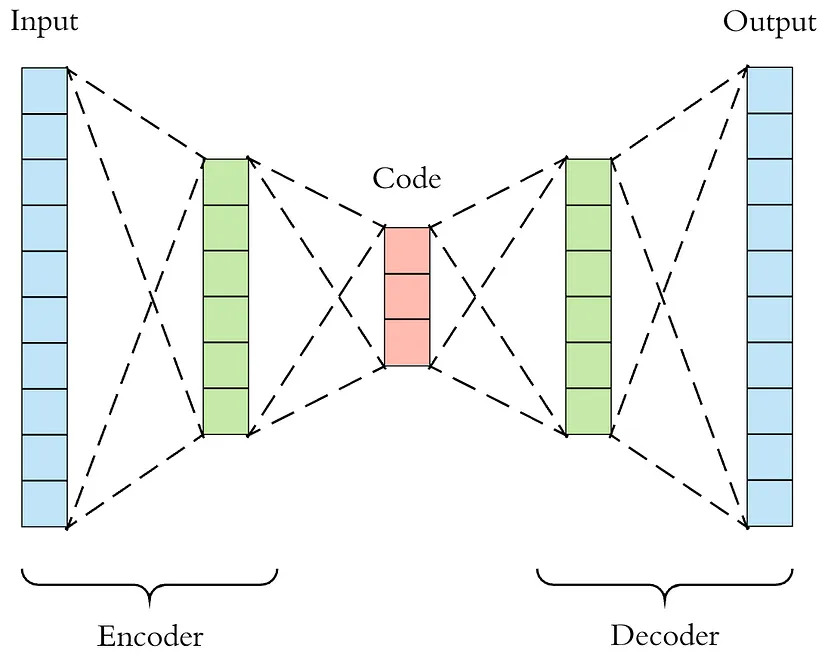
\includegraphics[scale=0.4]{autoencoding.jpg}

\textbf{Figure 5:} Typical autoencoding structure, from Towards Data Science\\[2\baselineskip]

\end{center}

\subsection{Word2Vec}

After obtaining vectors, Word2Vec uses the cosine similarity metric to measure the similarity of the words. Due to that, this architecture is similar to autoencoders, where there are encoder and decoder layers. If the cosine value of two words is 0, then words do not hold similarity. If the cosine value of two words is 1, then the words are overlapping. Due to that, the Word2Vec model is mostly used in semantic analysis. On the other hand, the main disadvantage of the Word2Vec model is that it can not handle vocabulary words well. The words that were not present in training data are called out of vocabulary words.  As Chandran stated (2020), a random vector representation is assigned for out-of-vocabulary words by Word2Vec, and they can be not optimal. Word2Vec constructs vectors with two methods: Skip-Gram and CBOW methods. Those two methods are discussed in previous chapters. Briefly, Skip-Gram generates surrounding words by the center word, while CBOW does the opposite: generating the center word by surrounding words. In the following application section, both Skip-Gram and CBOW models are used.

\section{Application}
In this section, Skip-Gram and CBOW are applied to The Divine Comedy by Dante Alighieri. Before applying models to The Divine Comedy, brief information about the dataset is given and then the dataset is prepared for the models.

\subsection{Information About the Dataset}
The Divine Comedy is an epic poem written by Italian poet Dante Alighieri in the 14th century. While it is considered one of the greatest works of literature, the poem is divided into three parts. Those three parts represent different realms of the afterlife and consist of Inferno (Hell), Purgatorio (Purgatory), and Paradiso (Paradise).

The Divine Comedy is chosen for this paper due to several reasons. Firstly and most significantly, The Divine Comedy is a voluminous work that consists of a wide range of characters, concepts, and names. Due to its rich vocabulary, it provides a great spectrum of words to use for the model. Secondly, The Divine Comedy has a great cultural significance for both European and world literature. Due to this importance, it has countless adaptations in various languages, and finding these adaptations is easier compared to other works of literature. Finally, The Divine Comedy explores fundamental aspects of human nature like sin, love, and redemption. The concepts explored in The Divine Comedy are mostly universal and due to that appear in different languages. Thanks to that, working on The Divine Comedy can show how language reflects universal concepts.

For this paper, versions of The Divine Comedy in different languages are used and the data is taken from \href{https://www.gutenberg.org/}{Project Gutenberg}. Six different versions of The Divine Comedy in different languages are used and those languages are \href{https://www.gutenberg.org/cache/epub/39181/pg39181-images.html}{Dutch}, \href{https://www.gutenberg.org/cache/epub/1004/pg1004-images.html}{English}, \href{https://www.gutenberg.org/cache/epub/12546/pg12546.html}{Finnish}, \href{https://www.gutenberg.org/cache/epub/8085/pg8085.html}{German}, and \href{https://www.gutenberg.org/cache/epub/1000/pg1000-images.html}{Italian}.

\subsection{Application}

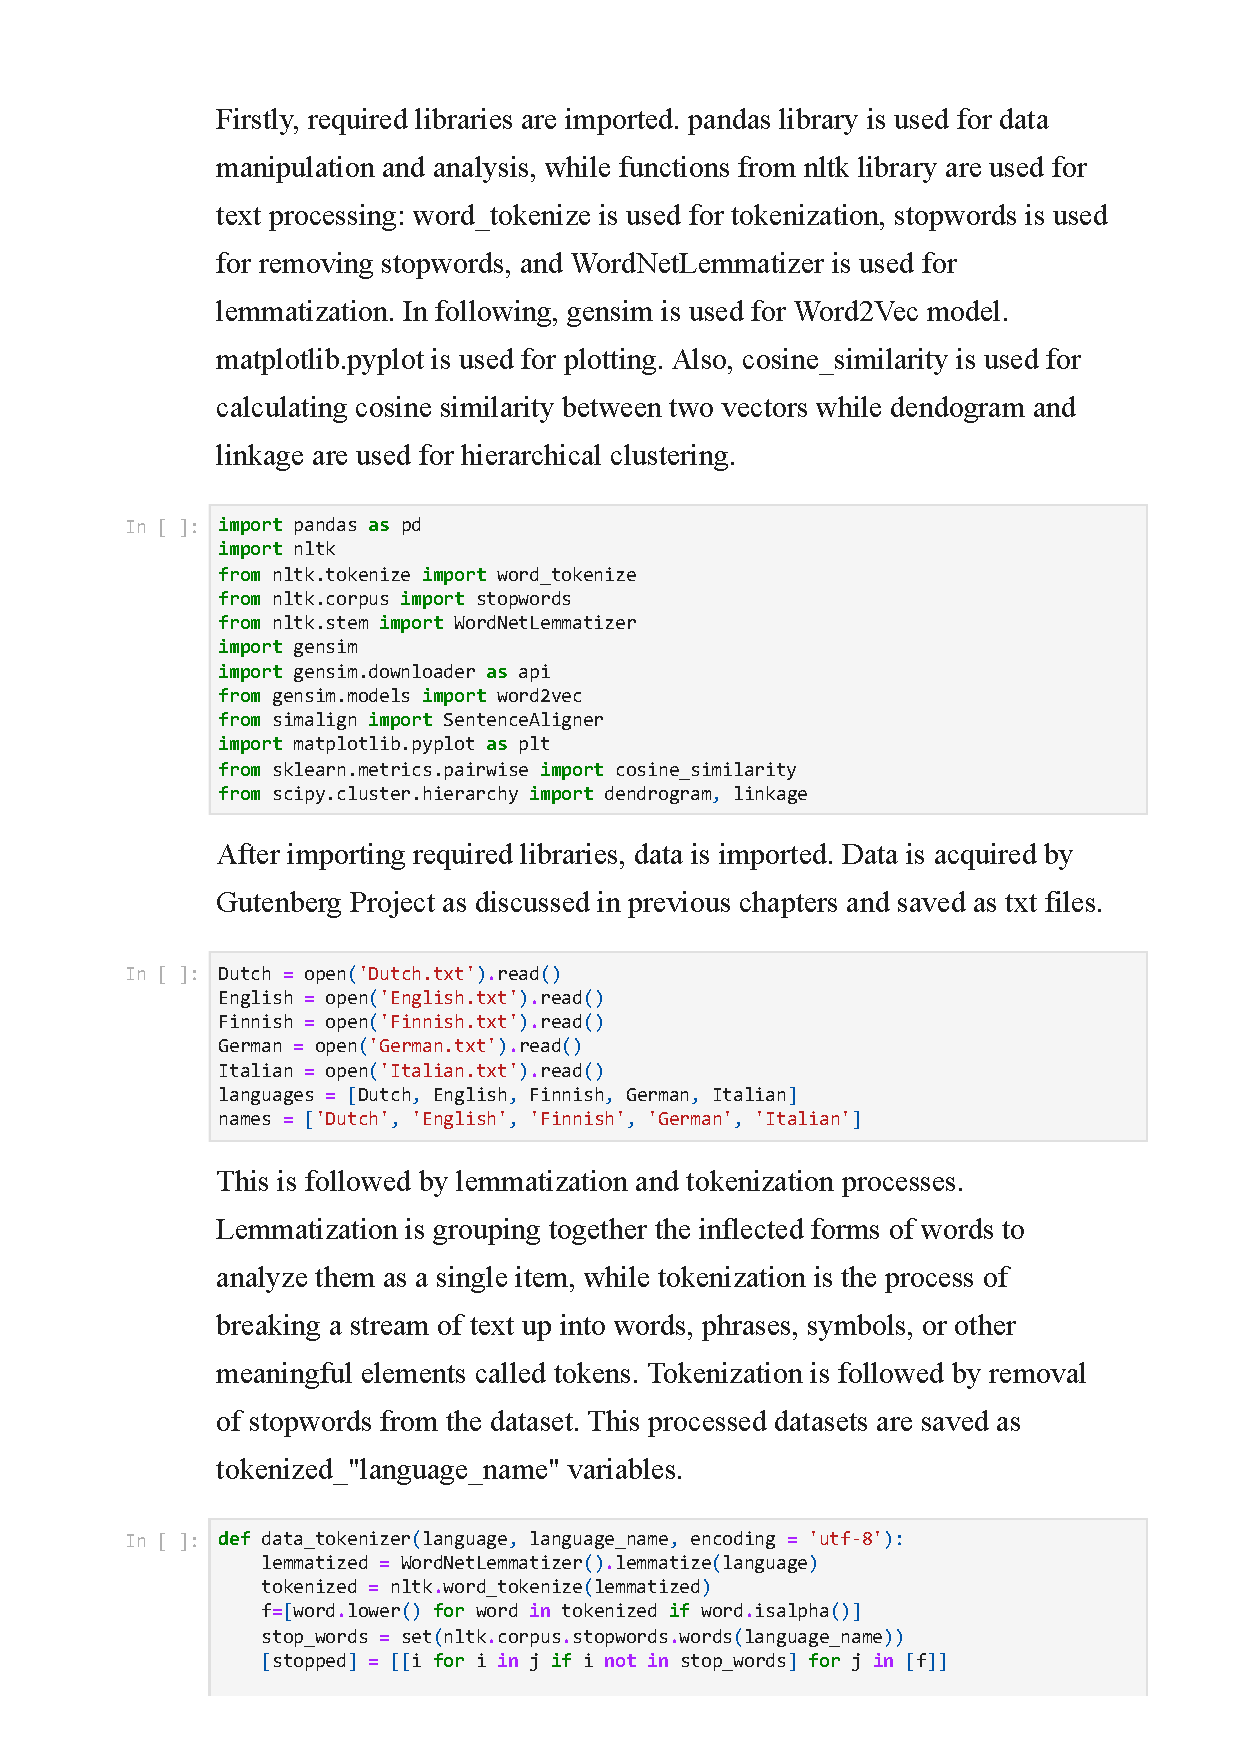
\includepdf[pages=-]{Application.pdf}

\section{Discussion}
All in all, two different dendrograms are obtained by Skip-Gram and CBOW in order. \textbf{Figure 7} visualize a dendogram as desired, while \textbf{Figure 8} partially succeeds this task.

If \textbf{Figure 7} is examined, It can be seen that Finnish, the only Uralic language in the dataset, is clustered differently from the rest of the dataset, while the other four Indo-European languages are clustered together. If these four languages are examined further, the only romance language Italian is also clustered further than the other three languages which are all Germanic. This clustering shows the relationship of languages correctly and It can be said that the Skip-Gram model succeeded in this task. In addition, English and Dutch are clustered closer to each other rather than German.

When moved to \textbf{Figure 8}, the only difference from the Skip-Gram dendrogram is the clustering of Italian. Instead of being clustered with other Indo-European languages, Italian is clustered with the Uralic language Finnish. Even though culturally and geographically there is no close relation between Finland and Italy, this clustering might be caused by the characteristic of the dataset or word-co-occurrence patters in the dataset. This can be tested by constructing a model with different datasets. Other than Italy, the CBOW model clustered languages the same as the Skip-Gram model.

\section{Conclusion}
To conclude, Dante Alighieri's Divine Comedy is studied in this paper as a dataset, and different word embedding techniques are used on it. Relationships of languages are investigated with the help of the most common words that occured in the dataset. To take this study further, one can study a dataset that contains more languages and investigate why Finnish and Italian are clustered together in the CBOW model.
\newpage
\begin{thebibliography}{7}
\bibitem{article}
Agarwal, N. (2022). \emph{The Ultimate Guide To Different Word Embedding Techniques In NLP}. KDnuggets. Retrieved from https://www.kdnuggets.com/2021/11/guide-word-embedding-techniques-nlp.html
\bibitem{english}
Alighieri, D. (1997). Divine Comedy, Longfellow's Translation, Complete (H. W. Longfellow, Trans.). Retrieved from https://www.gutenberg.org/cache/epub/1004/pg1004-images.html
\bibitem{Italian}
Alighieri, D. (1997). La Divina Commedia di Dante: Complete. Project Gutenberg. Retrieved from https://www.gutenberg.org/cache/epub/1000/pg1000-images.html
\bibitem{Finnish}
Alighieri, D. (2004). Jumalainen näytelmä. E. Leino (Trans.). Project Gutenberg. Retrieved from https://www.gutenberg.org/cache/epub/12546/pg12546.html
\bibitem{German}
Alighieri, D. (2005). Die Göttliche Komödie. Project Gutenberg. Retrieved from https://www.gutenberg.org/cache/epub/8085/pg8085.html
\bibitem{dutch}
Alighieri, D. (2012). Dante's Louteringsberg (H. J. Boeken, Trans.). Project Gutenberg. Retrieved from https://www.gutenberg.org/cache/epub/39181/pg39181-images.html




\bibitem{chandran}
Chandran, S. (2020). \emph{Introduction to Text Representations for Language Processing — Part 2}. Towards Data Science. Retrieved from https://towardsdatascience.com/introduction-to-text-representations-for-language-processing-part-2-54fe6907868
\bibitem{didl}
Dive Into Deep Learning. (n.d.). \emph{The Skip Gram Model}. Retrieved from https://d2l.ai/chapter\_natural-language-processing-pretraining/word2vec.html\#the-skip-gram-model
\bibitem{didl2}
Dive Into Deep Learning. (n.d.). \emph{The Continuous Bag of Words (CBOW) Model}. Retrieved from https://d2l.ai/chapter\_natural-language-processing-pretraining/word2vec.html\#the-continuous-bag-of-words-cbow-model
\bibitem{didl3}
Dive Into Deep Learning. (n.d.). \emph{Bidirectional Encoder Representations from Transformers (BERT)}. Retrieved from https://d2l.ai/chapter\_natural-language-processing-pretraining/bert.html\#bidirectional-encoder-representations-from-transformers-bert
\bibitem{gensim}
Gensim. (n.d.). \emph{Introducing: the Word2Vec Model}. Retrieved from
https://radimrehurek.com/gensim/auto\_examples/tutorials/run\_word2vec.html\#sphx-glr-auto-examples-tutorials-run-word2vec-py
\bibitem{glove}
Pennington, J. Socher R., Manning, C. D. (n.d.). \emph{GloVe: Global Vectors for Word Representation}. Retrieved from https://nlp.stanford.edu/projects/glove/
\bibitem{article2}
Kınık, D., Güran, A. (2021). TF-IDF ve Doc2Vec Tabanlı Türkçe Metin Sınıflandırma Sisteminin
Başarım Değerinin Ardışık Kelime Grubu Tespiti ile Arttırılması, \emph{Avrupa Bilim ve Teknoloji Dergisi}, 21, 323-332.
\bibitem{nationalgeo}
National Geographic. (2022). Retrieved from \emph{Family of Language}. https://education.nationalgeographic.org/resource/family-language/
\bibitem{simplilearn}
Simplilearn. (2023). \emph{What are Autoencoders? Introduction to Autoencoders in Deep Learning}. Retrieved from https://www.simplilearn.com/tutorials/deep-learning-tutorial/what-are-autoencoders-in-deep-learning
\end{thebibliography}
\end{document}